\documentclass[12pt]{standalone}
\usepackage[utf8]{inputenc}
\usepackage{tikz}
\usetikzlibrary{arrows.meta}
\usepackage{graphicx}

\begin{document} 
   \begin{tikzpicture}[font=\sffamily]
		\node[inner sep=0pt] (fig) at (0,0) {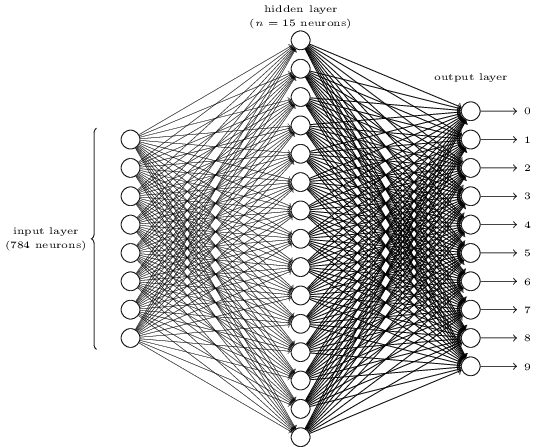
\includegraphics[]{neural_network.png}};
		\node[inner sep=0pt] (fig) at (-15,0) {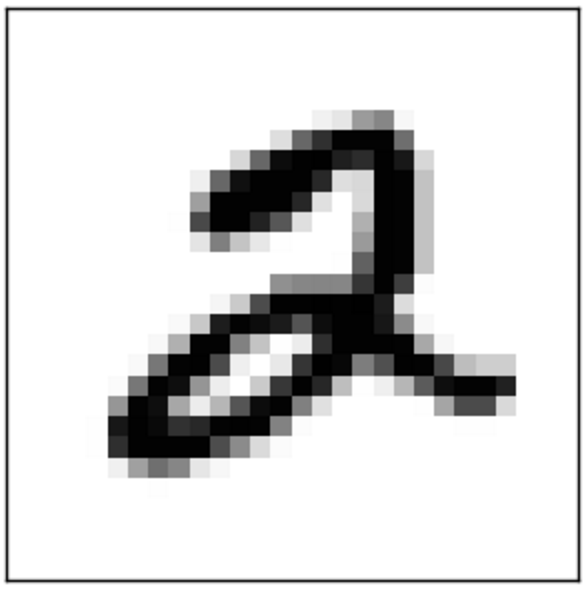
\includegraphics[]{mnist-2.png}};
		
		\node[] at (10.5,4) {(};
		\node[] at (10.5,3) {(};
		\node[] at (10.5,2) {(};
		\node[] at (10.5,1) {(};
		\node[] at (10.5,0) {(};
		\node[] at (10.5,-1) {(};
		\node[] at (10.5,-2) {(};
		\node[] at (10.5,-3) {(};
		\node[] at (10.5,-4) {(};
		\node[] at (10.5,-5) {(};
		
		\node[blue] at (11,4) {0.07};
		\node[blue] at (11,3) {0.12};
		\node[blue] at (11,2) {0.13};
		\node[blue] at (11,1) {0.15};
		\node[blue] at (11,0) {0.04};
		\node[blue] at (11,-1) {0.09};
		\node[blue] at (11,-2) {0.03};
		\node[blue] at (11,-3) {0.17};
		\node[blue] at (11,-4) {0.14};
		\node[blue] at (11,-5) {0.06};
		
		\node[] at (12.15,4) {- 0)$^2$ =};
		\node[] at (12.15,3) {- 0)$^2$ =};
		\node[] at (12.15,2) {- 1)$^2$ =};
		\node[] at (12.15,1) {- 0)$^2$ =};
		\node[] at (12.15,0) {- 0)$^2$ =};
		\node[] at (12.15,-1) {- 0)$^2$ =};
		\node[] at (12.15,-2) {- 0)$^2$ =};
		\node[] at (12.15,-3) {- 0)$^2$ =};
		\node[] at (12.15,-4) {- 0)$^2$ =};
		\node[] at (12.15,-5) {- 0)$^2$ =};
		
		\node[red] at (13.5,4) {0.0049};
		\node[red] at (13.5,3) {0.0144};
		\node[red] at (13.5,2) {0.0169};
		\node[red] at (13.5,1) {0.0225};
		\node[red] at (13.5,0) {0.0016};
		\node[red] at (13.5,-1) {0.0081};
		\node[red] at (13.5,-2) {0.0009};
		\node[red] at (13.5,-3) {0.0289};
		\node[red] at (13.5,-4) {0.0196};
		\node[red] at (13.5,-5) {0.0036};
	
   \end{tikzpicture}
\end{document} 